\chapter{Jet model based on a single knot}\label{chapter4}
\begin{figure}
\centering
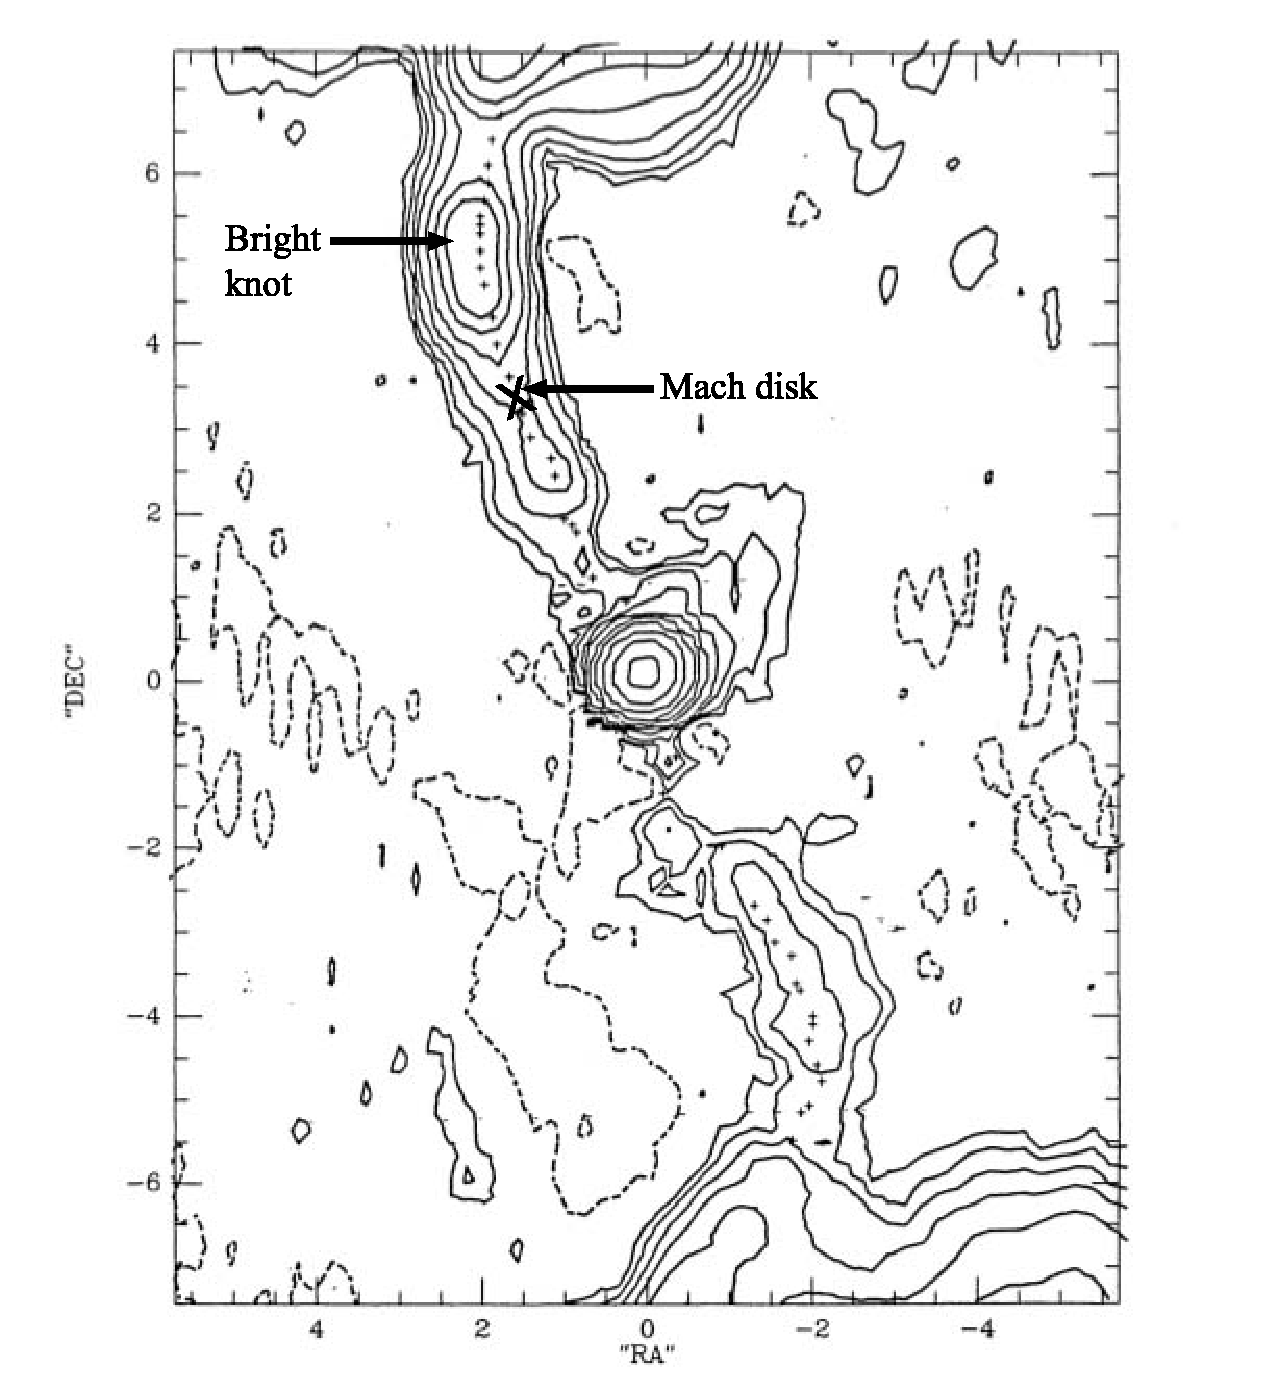
\includegraphics[width=\linewidth]{tp.eps}
\caption{Fig. 3 of \citet{taylor90}. Central 10~kpc jets of Hydra A. Contour levels are at 1.0, 2.0, 7.8, 15, 32, 51, 103, 208, and 417 mJy arc sec$^{-2}$. The bright knot is marked with black arrow. The location of the Mach disk (at approximately 6~kpc, marked by a $\times$) which I originally interpret as the reason for the bright knot, is also indicated.}
\label{f:morph}
\end{figure}

\begin{figure}
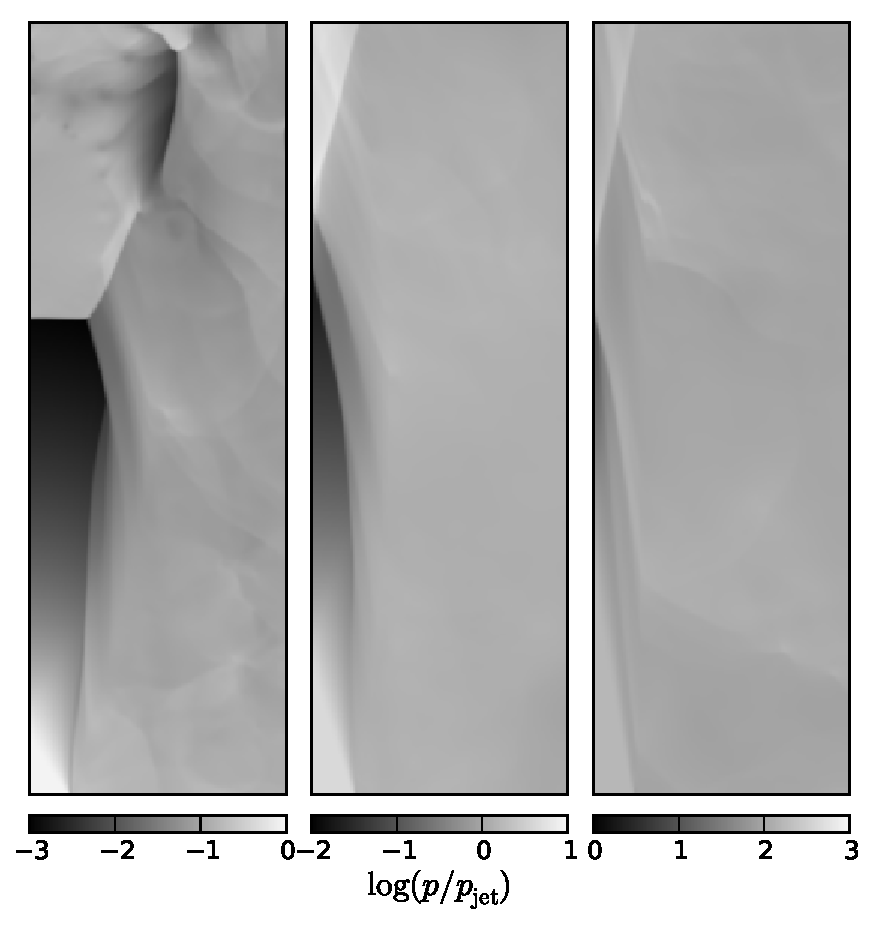
\includegraphics[width=\linewidth]{pss.eps}
\caption{Logarithmic pressure maps of the jet and ambient medium in the inner region of the 2D simulations. Left: A jet with an over-pressure ratio of 10 producing a Mach disk (Simulation Cvia). Middle: A jet with an over-pressure ratio of 5 producing a reconfinement shock. (Simulation Cviib) Right: A nearly pressure equilibrium jet ($p_{\rm jet}/p_{\rm a} = 2$) producing a very weak conical reconfinement shock (Simulation Cviic). Each panel has physical dimensions of $2\,\mathrm{kpc}\times6\,\mathrm{kpc}$.}
\label{pressure_comparison}
\end{figure}

%The first goal of this thesis is to understand the physics involved in the jet-ICM interaction within the central 10~kpc of the source Hydra A.  

My initial work on modelling Hydra A was based upon the published images of \citep{taylor90} in which a single bright knot is evident in the first 10~kpc of the northern jet. Consequently the work described here is based upon the production of a single bright knot in the first 10 kpc. Subsequent to this work, Prof, Gregory Taylor kindly provided a FITS image of Hydra A so that I could determine the brightness ratio of the northern and southern jets. When I contoured this image I realised that there are in fact two knots in the northern Hydra A jet (see Fig.~\ref{taylor}), first of which could with hindsight be faintly discerned in the original published images. Consequently, the following chapter contains a series of models devoted to the modelling of two knots. This chapter describes my work on the single knot interpretation. The comparison between the two models is of interest since it shows the different parameters that are obtained when different assumptions are made. 

%% Modify the following text to be consistent.
%I first focus the bright knot apparent at approximately 6 to 10~kpc of the northern jet (see Fig.3 of \citet{taylor90}). 
%Fig.~\ref{taylor} is produce later from the original 6~cm VLA data kindly provided by Professor Gregory Taylor which shows two inner knots at approximately 3.7~kpc and 7.0~kpc in the northern jet until it becomes turbulent. Therefore, the study presented in this chapter only consider the second knot. Moreover looking at Fig.3 of \citet{taylor90} I assume the southern edge of the second knot is at $\sim$6~kpc away from the black hole. 

My initial guess is that the bright knot in the northern jet is a consequence of a Mach disk at approximately 6~kpc produced by the interaction of an over pressured jet and the cluster environment. See \S~\ref{sec:reconf} for the description of reconfinement shock model of jet knots. Depending on the pressure ratio between the jet and the atmosphere, there are two different types of reconfinement shock structures that can occur: strong shocks perpendicular to the jet flow, often referred to as Mach disks, and conical shocks. Fig.~\ref{pressure_comparison} shows a comparison of the morphology of a jet that is significantly over-pressured (left panel), mildly over-pressured, and in nearly pressure equilibrium (right panel) with respect to the ambient medium. It is well known that a supersonic jet may display a sequence of conical shocks, also known as ``diamond shocks'', if the jet is over or under-pressured or in nearly pressure-equilibrium with respect to the ambient medium. The jet repeatedly expands and contracts towards the jet axis resulting in a sequence of conical shocks. When the pressure ratio of the jet and the atmosphere is sufficiently high (e.g., $p_{\rm{jet}}/p_{\rm{a}}\gtrsim10$), a Mach disk occurs normal to the flow. Such shocks occur in the following way: The propagation of the supersonic jet produces a lobe of shocked gas whose pressure is initially higher than the jet pressure. As the jet propagates, the lobe pressure decreases. When the lobe pressure becomes lower than the jet pressure, the jet expands rapidly sideways and the subsequent reconfinement produces a Mach disk. Behind the Mach disk, a transition to turbulence occurs, which is more rapid than that associated with conical shocks. A Mach disk is very disruptive; it drastically reduces the jet velocity in the inner section of the jet and also establishes a strongly sheared flow between the inner jet and its outer layer as shown in Fig. \ref{f:morph}. Oblique conical shocks are not as disruptive as the Mach disk. 

%\citet{norman82} first drew attention to the production of conical and normal shocks in over-pressured astrophysical jets.

%%%%%%%%%%%%%%%%%%%%%%%%%%%%%%%%%%%%%%%%%%%%%%%%%%%%%%%%%%%%%%%%%%%%%%%%
%
%												CODE AND SIMULATION PARAMETERS
%
%%%%%%%%%%%%%%%%%%%%%%%%%%%%%%%%%%%%%%%%%%%%%%%%%%%%%%%%%%%%%%%%%%%%%%%%
\section{Simulation Parameters} \label{code}

%%%%%%%%%% new table %%%%%%%%%%%%%4
\begin{table*}
%\begin{sidewaystable}
\caption{Simulation parameters. In all simulations, $r_{\rm{jet}}=0.38$ kpc.}
\centering
\begin{tabular}{l * {8}{c}}
\hline \hline
Model  & $p_{\rm{jet}}/p_{\rm{a}}$ & $\beta$ & $\chi$ & $\eta$ & $\phi$ (rad cm$^{-2}$) & $\Psi_{6\rm{cm}}$ (rad) & $\Psi_{20\rm{cm}}$ (rad) \\
\hline
    %%%%%%%%%% 		set A 	%%%%%%%%%%%%%%%
	\multicolumn{8}{c}{Set A, $P_{\rm{jet}}=1\times10^{45}$ erg s$^{-1}$} \\ 
	\hline
  	 Ai		&  10 & 0.09 & 1029 & $1.2\times10^{-1}$ &	$3.2\times10^{-2}$ 			&	1.14	 		&	12.63  \\
	Aii 	&  10 & 0.11 &  530  &  $6.0\times10^{-2}$ &	$1.6\times10^{-2}$	 		&	0.59	 		& 6.51	 \\
	Aii	&  10 & 0.13 &   301 & $3.4\times10^{-2}$ &	$9.2\times10^{-3}$ 	 		&	0.33 	 		&   3.69	 \\
	Aiv	&  10 &  0.15 &  182 & $2.0\times10^{-2}$ &	$5.6\times10^{-3}$			&	0.20	 		& 	2.23	\\
	Av	&  10 & 0.17 &  116 & $1.3\times10^{-2}$  &	$3.6\times10^{-3}$	  		&	0.13			&  1.42	\\
	Avi 	&  10 &  0.19   &    76 &  $8.5\times10^{-3}$ &	$2.3\times10^{-3}$ 			& 0.08	  		& 0.93 \\
	Avii	&  10 &  0.21   &    51 &  $5.7\times10^{-3}$ &	$1.6\times10^{-3}$			&   0.06			& 0.63	 \\
	\hline
	%%%%%%%%%% 		set B 	%%%%%%%%%%%%%%%
	\multicolumn{8}{c}{Set B, $P_{\rm{jet}}=3\times10^{44}$ erg s$^{-1}$} \\ 
	\hline 
	Bi	&10 & 0.04 & 3143  & $3.5\times10^{-1}$	&	$9.7\times10^{-2}$			& 3.47	 	& 38.59 \\
	Bii 	&  10 & 0.05 &   1447 & 	$1.6\times10^{-1}$ &	$4.4\times10^{-2}$	 	& 1.60	 	& 17.76	\\
	Biii	&  10 & 0.06 &   743 &  	$8.3\times10^{-2}$	& $2.3\times10^{-2}$		& 0.82	 	& 9.12	 \\
	Biv	& 10 &  0.07 &  409 &  	$4.6\times10^{-2}$	& $1.3\times10^{-2}$	 	& 0.45	 	& 5.02	  \\
	Bv	& 10 & 0.08 &  234 & 	$2.6\times10^{-2}$	&	 $7.2\times10^{-3}$ 		&	0.25	 	& 	2.87	 \\
	Bvi	&  10 &  0.09   &   136  &  $1.5\times10^{-2}$	& $4.2\times10^{-3}$	 	&	0.15	  	& 1.67	 \\
	Bvii	&  10 &  0.10   &    79 &   $8.8\times10^{-3}$	& $2.4\times10^{-3}$ 		& 	0.09	  	& 	0.97	 \\
	\hline
%\begin{comment}
	%%%%%%%%%% 		set C 	%%%%%%%%%%%%%%%
        \multicolumn{8}{c}{Set C, $P_{\rm{jet}}=3\times10^{45}$ erg s$^{-1}$} \\
        \hline
	Cia	&10 & 0.25 & 135 & $1.5\times10^{-2}$  & 	$4.1\times10^{-3}$			&	0.15		 	& 	1.66	 \\
	
   Cib  &5 & 0.25 & 301 & $1.7\times10^{-2}$  	&	$4.6\times10^{-3}$ 	   			&	0.17	 		& 	1.85		\\
   Cic  &2 & 0.25 & 800 & $1.8\times10^{-2}$   	&	$4.9\times10^{-3}$	 			&	0.18	  		&	1.96		\\	
    
	Ciia 	& 10 & 0.30 &  71 &  $7.9\times10^{-3}$ 	& $2.2\times10^{-3}$	 		&	0.08	 		& 0.87 	  	\\
    
    Ciib    &5 & 0.30 & 164 & $9.1\times10^{-2}$  & $2.5\times10^{-3}$ 	  			&	0.09	 		& 1.01	 \\
    Ciic    &2 & 0.30 & 442 & $1.0\times10^{-3}$  	&	$2.7\times10^{-3}$    		&	0.10		& 1.09	 \\

	Ciiia 	& 10 & 0.35 &  40 &  $4.5\times10^{-3}$  	& $1.2\times10^{-3}$	 		&	0.04			& 0.49  \\

   Ciiib    &5 & 0.35 & 96 & $5.4\times10^{-2}$ 	&	$1.5\times10^{-3}$ 	   			&	0.05			&	0.59		\\
    Ciiic   &2 & 0.35 & 263 & $5.9\times10^{-3}$   &	$1.6\times10^{-3}$ 	 			&	0.06	  		& 0.64		\\

	Civa	& 10 &  0.40 & 23 & $2.6\times10^{-3}$ 	& $7.2\times10^{-4}$			&	0.03	    	& 0.29	 \\

    Civb    &5 & 0.40 & 59 & $3.3\times10^{-2}$  	& $9.0\times10^{-4}$	   		&	0.03		& 0.36	 \\
    Civc  &2 & 0.40 & 165 & $3.7\times10^{-3}$   	& $1.0\times10^{-3}$	  		&	0.04	 	& 0.41	 \\

	Cva 	& 10 & 0.45 &  14 & $1.6\times10^{-3}$	& $4.3\times10^{-4}$	 		&	0.02   	&	0.17   \\

    Cvb    &5 & 0.45 & 37 & $2.1\times10^{-2}$   	& $5.7\times10^{-4}$	 		&	0.02  	&	 0.23 \\
    Cvc   &2 & 0.45 & 107 & $2.4\times10^{-3}$  	& $6.6\times10^{-4}$	 		&	0.02  	& 0.26	 \\

	Cvia & 10 & 0.50 & 8 &  $9.3\times10^{-3}$ 	& $2.6\times10^{-4}$	 		&	0.01	 	& 0.10	 \\

  Cvib    &5 & 0.50 & 24 & $1.4\times10^{-2}$   	&  $3.7\times10^{-4}$	 		&	0.01 		&	0.15	 \\
   Cvic    &2 & 0.50 & 71 & $1.6\times10^{-3}$   	& $4.4\times10^{-4}$	  		&	0.02	 	& 0.18	 \\

	Cviia	& 10 & 0.55 & 5 & $5.3\times10^{-4}$ 	& $1.5\times10^{-4}$	 		&	0.01  	& 0.06	 \\

   Cviib   &5 & 0.55 & 16 & $8.7\times10^{-4}$  	& $2.4\times10^{-4}$	   		&	0.01  	&	 0.10 \\
   Cviic   &2 & 0.55 & 48 & $1.1\times10^{-3}$  	& $3.0\times10^{-4}$	 		&	0.01  	& 0.12 		\\
\hline
	
%\tablefootnote{index $p$ is used to separate the parallel opening jet models presented here and the conically expanding jet models presented in the following chapter.}
\end{tabular}
\label{simulation_parameters}
%\end{sidewaystable}
\end{table*}



%%%%%%%%%%%%%%%%%%%%%%%%%%%%%%%

%\begin{table*}
\begin{sidewaystable}
\caption{Inferred jet velocities for Hydra A northern jet as a function of jet power and pressure ratio}
\begin{tabular}{l * {16}{c}}
\hline \hline
$P_{\rm{jet}}$(erg s$^{-1}$) & $p_{\rm{jet}}/p_{\rm{a}}$  & $\chi$ & $\eta$ & $\beta$ \\
\hline
 $3\times10^{44}$ & 10 & 1447 & $1.6\times10^{-1}$ & 0.05 \\ 
 $1\times10^{45}$ & 10 &  116 & $1.3\times10^{-2}$   & 0.17 \\ 
 $3\times10^{45}$ & 10 &   14 & $1.6\times10^{-3}$ & 0.45 \\ 
 $3\times10^{45}$ &  5 &   59, 37, 24, 16 & $(3.3, 2.1, 1.4, 0.1)\times10^{-2}$ & 0.4-0.55 \\ 
  $3\times10^{45}$ &  2 &   800, 442, 263, 165, 107, 71, 48  & $(1.8, 0.1, 0.6, 0.4, 0.2, 0.2, 0.1)\times10^{-2}$ & 0.25-0.55 \\ 
\end{tabular}
\label{inferred_jet_velocities}
\end{sidewaystable}
%\end{table*}


%For the simulations I use the the publicly available PLUTO code \citep{mignone07} to calculate two dimensional axisymmetric hydrodynamic models of the jet-ICM interaction in Hydra A. Since some of the models include relativistic velocities I use the relativistic hydrodynamic (RHD) module available in PLUTO. 

In the models presented here, I initialise a parallel jet into the computation domain following \citet{sutherland07, wagner11}.  The $(r, z)$ computational domain for the two dimensional axisymmetric simulations is a cylinder of radius $r=25$ kpc and height $z=50$ kpc. Using a stretched grid I define a high resolution grid ($1600 \times 160$ cells) within the central $20\,\mathrm{kpc}\times2\,\mathrm{kpc}$ region, giving us 30 cells across the jet, and a lower resolution in the outer regions. I impose an axisymmetric boundary condition for the boundary $r=0$, and a reflective boundary condition for $z=1$.  The remaining boundaries are set to outflowing boundaries.

The jet is initiated within a quarter circle with radius 0.38 kpc and centre at $(r, z) = (0, 1)~kpc$. The time invariant jet parameters are jet power $P_{\rm{jet}}$, jet radius $r_{\rm{jet}}$, inlet jet pressure $p_{\rm{jet}}$, inlet jet velocity $\beta$, and the proper density parameter 
\begin{equation}
\chi =  \frac{\rho_{\rm jet} c^2}{\varepsilon + p_{\rm jet}} = (\gamma -1)\rho_{\rm{jet}}c^2/\gamma p_{\rm{jet}}
\end{equation}
where $c$ is the speed of light, $\varepsilon$ is the internal energy density, and $\gamma$ is the polytropic index. The jet velocity vectors at the jet base are parallel to the positive $z$--direction.
%$\chi = (\gamma -1)\rho_{\rm{jet}}c^2/\gamma p_{\rm{jet}}$, where $\gamma$ is the polytropic index. The jet velocity vectors at the jet base are parallel to the positive $z$--direction.

%I use the \citet{taub1948a} equation of state, a quadratic approximation to the exact Synge--J\"{u}ttner relativistic perfect gas equation of state \citep{juttner1911a,synge1957a}, which yields $\gamma\rightarrow5/3$ in the low temperature limit, and $\gamma\rightarrow4/3$ in the high temperature limit. Because the radiative cooling time of the ambient gas and the synchrotron cooling time of the jet plasma is large compared to the simulation time (which is equivalent to the jet crossing time), I do not include radiative cooling in the simulations.

Let $A_{\rm{jet}}(=\pi r^2_{\rm{jet}}$) be the jet cross-sectional area and $\Gamma=(1-\beta^2)^{-1/2}$ be the jet Lorentz factor. Then the jet kinetic power is given by \citet{sutherland07}:
\begin{equation}
P_{\rm{jet}} = \frac{\gamma}{\gamma -1} c p_{\rm{jet}}\Gamma^2\beta A_\mathrm{jet}\left(1+\frac{\Gamma -1}{\Gamma}\chi\right)\:.
\label{jet_power}
\end{equation}
We determine the density parameter by solving Eqn.~\eqref{jet_power}:
\begin{equation}
\chi = \frac{\Gamma}{\Gamma -1}\left( \frac{\gamma-1}{\gamma}\frac{P_{\rm{jet}}}{c p_{\rm{jet}} \Gamma^2\beta A_{\rm{jet}}} -1 \right)\:.
\label{chi2}
\end{equation}

The initial conditions for the ambient medium representing the hot ICM surrounding Hydra A are the hydrostatic thermodynamic profiles found in \S~\ref{s:cluster}. The ratio, $\eta =\rho_{\rm jet}/\rho_{\rm  a}$, of the jet to ambient density is always an important parameter in jet theory and since I am allowing for a significant thermal component in the simulations it is important to estimate this parameter. If $T$ is the core temperature of the cluster atmosphere, $\rho_{\rm a}$ and $p_{\rm a}$ are the ambient density and pressure at the jet inlet, $k_B$ the Boltzmann constant and $m$ be the atomic mass unit, $\eta$ is given by 
\begin{equation}
\eta = \frac{\rho_{\rm{jet}}}{\rho_{\rm{a}}} = \chi \frac{\gamma}{\gamma-1}\frac{p_{\rm{jet}}}{p_{\rm{a}}}\frac{k_BT}{\mu m c^2}\:.
\label{eta}
\end{equation}
Equation~(\ref{chi2}) for $\chi$ and equation~(\ref{eta}) for $\eta$ typically lead to values of $\chi \gg 1$ (especially for low velocities) and correspondingly large values of $\eta \approx 10^{-2}$ in comparison to the typical value for AGN jets ($\eta \approx 10^{-4}$). The implications of this are discussed further below.

The simulations presented in the next section cover an extensive region in parameter space. The simulation parameters that are varied, and the ranges they span are: the jet power, $P_\mathrm{jet}=1\times10^{45}$, $3\times10^{44}$, $3\times10^{45} \> \rm erg \> s^{-1}$, the ratio of the jet pressure to that of the atmosphere at the jet base $p_{\rm{jet}}/p_{\rm{a}}=2, 5, 10$, and the jet velocity in units of the speed of light $\beta=0.04 - 0.55 \> c$, are presented in Table \ref{simulation_parameters}. The range in jet velocity is restricted to fairly low values because of the results presented in \S~\ref{s:sims}: the location of the first internal jet shock constrains the velocity to relatively low values. 

%In the model names I use an index $p$ (p for parallel opening jet) to separate the models for the conically expanding jets presented in the subsequent chapter. 

The jet radius is fixed at $r_\mathrm{jet}=0.38$ kpc. This value is measured from the deconvolved FWHM at approximately 1~kpc from the core of the northern jet. Some derived parameters, namely the density parameter $\chi$, the density ratio $\eta$ of the jet and the atmosphere at the jet base, the rotation measure (RM) $\phi$, and the Faraday rotation angle $\Psi$ at 6 cm ($\Psi_\mathrm{6cm}$) and 20 cm ($\Psi_\mathrm{20cm}$) are also presented in Table \ref{simulation_parameters}. The rotation measure and Faraday rotation of the central jet with electron density $n_\mathrm{\mathrm e,jet}$(=$\rho_{\mathrm jet}$(1 + 2 $n_{\mathrm He}$/$n_{\mathrm H}$)/u(1 + 4$n_{\mathrm He}$/$n_{\mathrm H}$), where $u$ is an atomic mass unit), magnetic field along the line of sight $B_z$ (we use $35 \> \mu\,\mathrm{G}$, approximately the minimum energy magnetic field near the jet base), differential plasma depth $dl$, jet radius $R_{\rm{jet}}$, total plasma depth $L=2R_{\rm{jet}}$, and wavelength $\lambda$ are calculated from
\begin{eqnarray}
\phi &=& 8.1\int n_\mathrm{e,jet} B_z dl \quad \rm rad \, cm^{-2} \nonumber \\
&=& 8.1\times10^{-5}\, \left(n_{e, jet}\right) \left(\frac{B_z}{\mathrm{\mu G}}\right)  \left(\frac{2R_{\rm{jet}}}{\mathrm{kpc}} \right) \rm rad \, cm^{-2}
\end{eqnarray}
where the units of $B_z$ and $l$ are Gauss and cm, respectively. The total Faraday rotation through the jet is given by:
\begin{equation}
\Psi_{\rm rad} = \phi \lambda^2 \:.
\end{equation}

%The rotation measure and Faraday rotation angle of the central jet with electron density $n_\mathrm{e,jet}$, ambient electron density $n_\mathrm{e,a}=0.07$ (estimated from the ICM density profile), magnetic field along the line of sight $B_\parallel$ (we use $60 \> \mu\,\mathrm{G}$, approximately the minimum energy magnetic field near  the jet base),
%differential plasma depth $dl$, jet radius $R_{\rm{jet}}$, total plasma depth $L=2R_{\rm{jet}}$, and wavelength $\lambda$ are calculated from
%\begin{eqnarray}
%\phi_{\rm rad \, cm^{-2}} &=& 81 \int n_\mathrm{e,jet} B_z dl \nonumber \\
%&=& 0.081\,n_\mathrm{e,a} \left(\frac{\eta}{10^{-2}}\right) \left(\frac{B_z}{10^{-5}\,\mathrm{G}}\right)  \left(\frac{2R_{\rm{jet}}}{\mathrm{kpc}} \right) \: 
%\end{eqnarray}
%and
%\begin{equation}
%\Psi_{\rm rad} = \phi \lambda^2 \:.
%\end{equation}



I calculate these quantities as an additional check to ensure that the jet parameters are consistent with the fact that the jets are polarised along their length. The internal Faraday rotation should be much less than unity for consistency between the models and the observations. Note however, that the values given in Table~\ref{simulation_parameters} are maximum values and do not take into account the angle between the magnetic field and the line of sight, the possibility that the magnetic field may be sub-equipartition and the occurrence of field reversals.

I group the runs into three sets as set out in Table \ref{simulation_parameters}; Set A groups simulations with a jet kinetic power of $1\times10^{45} \> \rm erg \> s^{-1}$, which is the fiducial value adopted as discussed in \S~\ref{jet_kinetic_power}; Sets B and C group simulations with a jet kinetic powers of $3 \times 10^{44} \> \rm erg \> s^{-1}$ and 
$3 \times 10^{45} \> \rm erg \> s^{-1}$, respectively.   

It is evident from Eqns.~\eqref{chi2} and \eqref{eta}, that the dependence of the density parameter, $\chi$, and the density ratio, $\eta$, on the other jet parameters have implications for the allowable range of the pressure ratio $p_{\rm{jet}}/p_{\rm{a}}$. For $P_\mathrm{jet}=1\times10^{45} \> \rm erg s^{-1}$ and $3\times10^{44} \> \rm erg s^{-1}$ (simulation set A and B), the density ratio $\eta$ is too large for $p_{\rm{jet}}/p_{\rm{a}}<10$. A jet with too large a value of $\eta$ pierces the atmosphere with very little lateral expansion; the back-flowing jet plasma does not form a wide lobe, inconsistent with observations. Therefore there are fewer models in simulation set A and B, while in set C I can explore a more extensive  range of pressure ratios $2\leq p_{\rm{jet}}/p_{\rm{a}}\leq10$. Nevertheless, in most runs, the value of 
$\eta$ is still 10 to 100 times higher than the typical light jet assumption of  $\eta \sim 10^{-4}$ -- $10^{-3}$. This could indicates that the jet entrained a substantial amount of ambient material. For example, it is possible that the jet has interacted strongly with HI gas near the radio core, detected by \citet{dwarakanath95}.

%%%%%%%%%%%%%%%%%%%%%%%%%%%%%%%%%%%%%%%%%%%%%%%%%%%%%%%%%%%%%%%%%%%%%%%%
%
%									Simulation Results
%
%%%%%%%%%%%%%%%%%%%%%%%%%%%%%%%%%%%%%%%%%%%%%%%%%%%%%%%%%%%%%%%%%%%%%%%%

\section{Simulation Results}\label{s:sims}
%\begin{enumerate}

In this section I present the results of two dimensional axisymmetric hydrodynamic simulations of the interaction of the Hydra A radio jets with the ICM. I have conducted a large number of simulations to cover the parameter space described in table~\ref{simulation_parameters}. I first describe the association of the bright knot in the northern side of Hydra A with a transition to turbulence. As noted above a possible model for the bright knot and the turbulent transition is that it is the result of a normal shock (Mach disk). However, this remains to be confirmed by three dimensional simulations and I also describe here how conical shocks in the case of a less over-pressured jet may also explain these features. I then turn to the results of the parameter space study that enable us to constrain the jet velocity and other jet parameters by the location at which the first jet shock develops.
%\end{enumerate}

%%%%%%%%%%%%%%%%%%%%%%%%%%%%%%%%%%%%%%%%%%%%%%%%%%%%%%%%%%%%%%%%%%%%
%
%		MORPHOLOGICAL STRUCTURES: BRIGHT KNOT AND THE TURBULENT TRANSITION
%
%%%%%%%%%%%%%%%%%%%%%%%%%%%%%%%%%%%%%%%%%%%%%%%%%%%%%%%%%%%%%%%%%%%%
\subsection{Morphological Structures: The Bright Knot in the Northern Jet and the Transition to Turbulence}\label{morphological_structure}
\begin{figure*}
\centering
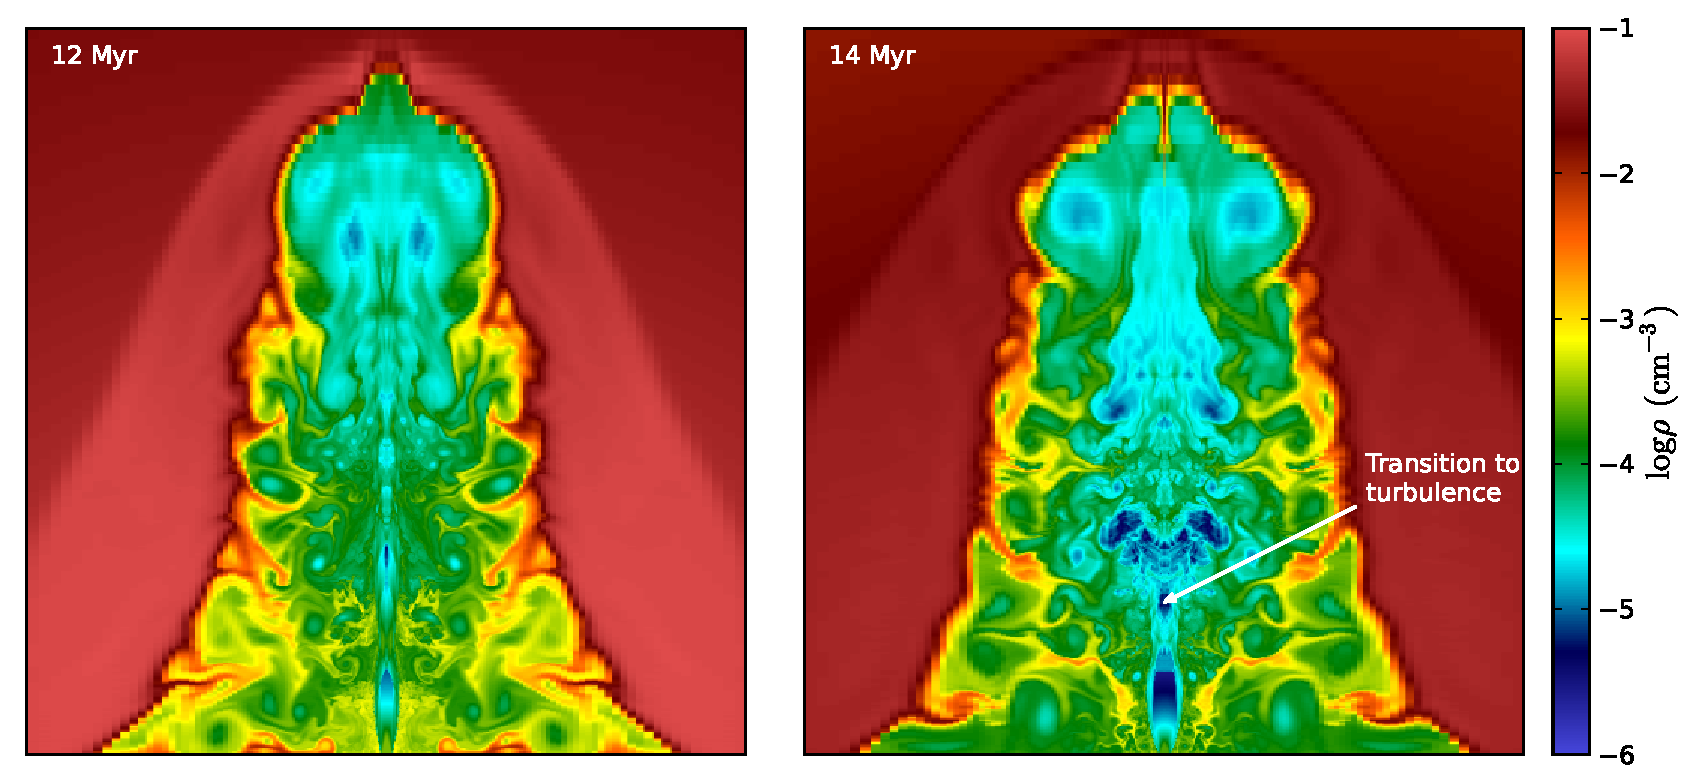
\includegraphics[width=\linewidth]{pls.eps}
\caption{Logarithmic density maps for simulations with a less over-pressured jet (run Cvb) and a sfignificantly over-pressured jet (run Cva). The comparison shows how the lobe structure differs for conical reconfinement shocks (left) and Mach disks (right), the latter being more effective in decelerating the jet and causing a turbulent transition. The dimension in each panel are ($50\,\mathrm{kpc}\times50\,\mathrm{kpc}$).}
\label{shock_comparison}
\end{figure*}
%It is possible that the northern jet undergoes a transition to turbulence associated with a Mach disk, while the southern jet transitions more gradually to turbulence via deceleration through conical reconfinement shocks


\begin{figure}
\centering
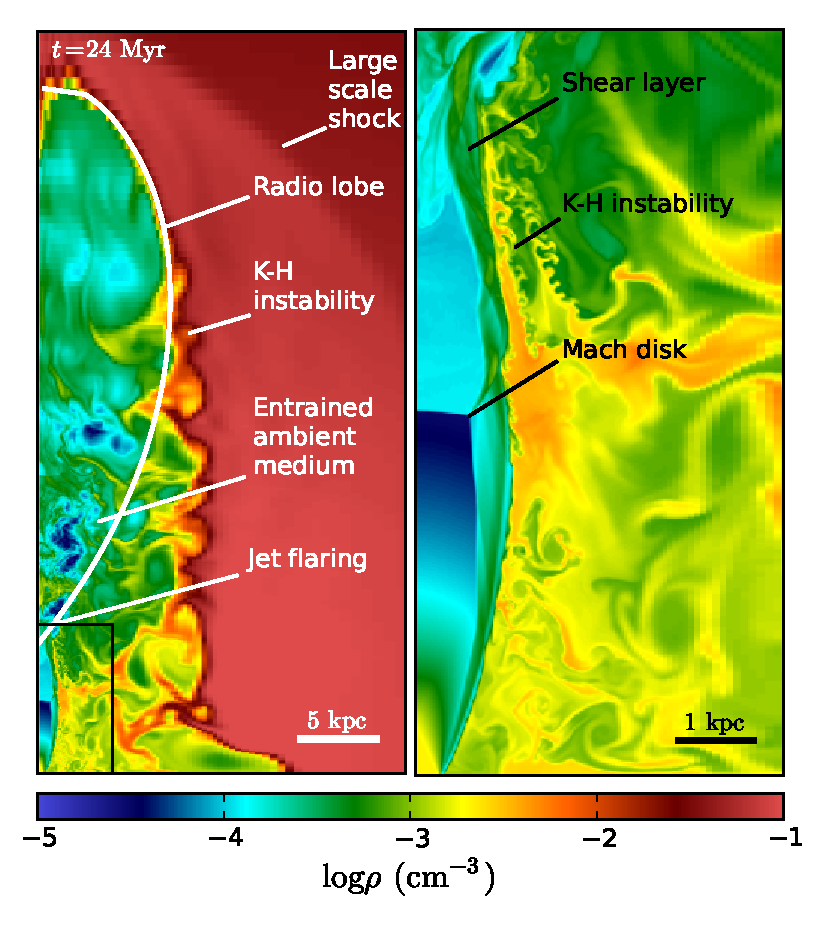
\includegraphics[width=\linewidth]{pbm.eps}
\caption{Logarithmic density map snapshot for run Av at $24\,\mathrm{Myr}$, labelling the main features of the jet-ICM interaction seen in simulations that exhibit a Mach disk. The right panel is a magnification of the central region marked with a box in the left panel.}
\label{f:morph}
\end{figure}


Fig. \ref{shock_comparison} shows two different lobe structures, one fed by a jet displaying shock diamonds (left panel), the other fed by a jet containing a Mach disk (right panel). These are snapshots from runs Cvb and Cva, respectively. Here two completely different types of jet and lobe morphology are seen. For the case of a less over-pressured jet ($p_{\rm{jet}}/p_{\rm{a}}=5$, run Cvb) the jet reconfinement proceeds through a series of shock diamonds. The jet remains coherent well inside the lobe and a number of conical shocks mediate a gradual transition to turbulence. In the other case of a jet over-pressured significantly by a factor of 10 (run Cva, right panel), the reconfinement results in a Mach disk. Although the association of a Mach disk with the northern jet bright knot consistently explain the morphology of the northern jet, I do not completely disregard the possibility of the association of a conical shock with the bright knot. Hence, in the following I determine the location of the first shock, either conical or normal, when I examine the dependence of the location of the northern bright knot on jet velocity.

%We see a violent transition to turbulence associated with the  disruptive Mach disk. These morphological features suggest that i) the northern jet of Hydra A is associated with a Mach disk, which causes both the bright knot and the subsequent rapid turbulent transition, and ii) the southern Hydra A jet can be explained by a more coherent jet associated with conical shocks which mediate a less violent turbulent transition. The association of a Mach disk and conical shocks with the northern and southern jet respectively, is also supported by the presence of the bright knot in the northern side and lack of a corresponding feature in the southern side. The increase in particle density and magnetic field associated with  oblique conical shocks are not as strong as the increase associated with a mach disk. The bright knot inside the southern lobe may be associated with a shock produced as the curved supersonic jet hits the cavity wall and abruptly changes direction. 


Fig. \ref{f:morph} shows the density image of the simulation Av at 24 Myr. I select this particular model as the fiducial model for the jets of Hydra A with a jet kinetic power of $P_\mathrm{jet}=1\times10^{45}\,\mathrm{erg}\,\mathrm{s}^{-1}$, because it clearly reproduces the transition of the jet to a turbulent plume at $\sim10$ kpc as indicated by the observations of the Hydra A northern jet. While this simulation snapshot represents the earliest phase of the development of the Hydra A plumes, I will assume that it is indicative of the dynamics in the inner $\sim10$ kpc of the jet during the subsequent evolution of the source. 

In this simulation, a Mach disk appears at $\sim6$ kpc from the jet inlet. I associate this Mach disk with the bright knot in the Hydra A northern jet. The shock-accelerated electrons and the compression of the magnetic field increase the synchrotron emission immediately behind the Mach disk and produce a bright radio knot. Downstream of the Mach disk, the jet flow is further decelerated and  becomes turbulent. The deceleration distance behind the Mach disk is $\sim 4$ kpc, in agreement with the observed distance between the bright knot at $\sim6$ kpc and the beginning of the turbulent plume at a distance of $\sim10$ kpc from the radio core. 

%The position of the Mach disk at $\sim6$ kpc in the Hydra A northern jet is consistent with the theoretical prediction of the position of the first reconfinement shock by \citet{stawarz06}. In their study of knot HST-1 in the M 87 jet they use the relativistic Rankine-Hugoniot shock jump condition to estimate the position of the first reconfinement shock. They assume that the jet is initially advancing freely and begins to reconfine at a location $r_1$, at which point it is in pressure equilibrium with the atmosphere ($p_1/p_{\rm{a}}=1$, where $p_1$ is the jet pressure at $r_1$ and $p_{\rm a}$ is the ambient pressure). In the case of Hydra A jets I estimate the starting point of the reconfinement $r_1$ by using the pressure ratio of the jet to the atmosphere at the jet inlet of the fiducial model Av ($p_{\rm{in}}/p_{\rm{a}}=10$, where $p_{\rm{in}}$ is the jet pressure at the inlet), and the jet inlet in the simulations is at a distance $r_{\rm{in}}\approx1\ \rm{arcsec}\approx1.1$ kpc from the centre of the galaxy.
%\begin{equation}
%\frac{p_1}{p_\mathrm{in}} = \frac{p_1}{p_\mathrm{a}}\frac{p_\mathrm{a}}{p_\mathrm{in}}= 1 \times \frac{1}{10} = \left(\frac{r_1}{r_\mathrm{in}}\right)^{-2\gamma}\:.
%\label{reconfinement}
%\end{equation} 
%
%We obtain $r_1=2.2$ and 2.6 kpc for a non-relativistic particle dominated jet ($\gamma=5/3$ and $\beta_2/\beta_1=1/4$) and a relativistic particle dominated jet ($\gamma=4/3$ and $\beta_2/\beta_1=1/7$) respectively. 
%
%For a jet plasma with polytropic index $\gamma$, an ambient pressure profile $p_{\rm{a}}\propto r^{-\delta}$ (where $\delta$ is the slope of the pressure profile), pre-shock velocity $\beta_1$ and post-shock velocity $\beta_2$ the analytical model for the position of the first reconfinement shock, $r_{\rm{c}}$ provided by \citet{stawarz06} is
%\begin{equation}
%r_c = r_1\left[ \frac{(2-\delta)^2(1-\beta_2/\beta_1)\gamma}{(\gamma-1)^2}\right]^{1/(2-\delta)}\:.
%\label{stawarz_reconfinement}
%\end{equation}
%
%From the atmosphere pressure profile derived in \S~\ref{s:cluster}, I estimate that $\delta=0.15$ at $\sim 6$ kpc. Solving equation~(\ref{stawarz_reconfinement}) I obtain $r_{\rm{c}}\approx7.5$ kpc for non-relativistic particle dominated jet and $r_{\rm{c}}\approx 18 \, \rm kpc$ for relativistic particle dominated jet. The position of the first reconfinement shock at $\sim 7.5 \, \rm kpc$ for the non-relativistic particle dominated jet is reasonably consistent with the result of the fiducial model Av, a Mach disk at $\sim 5 \, \rm kpc$ from the jet inlet i.e, at $\sim 6 \, \rm kpc$ from the galaxy centre. 
%
%This result reinforces the likelihood of higher values of $k$, say $k \sim 10$, as found in \S~\ref{s:p_res} and the likelihood that the jet is dominated by non-relativistic particles.

Other standard features of  simulation Av include a large-scale bow-shock advancing through the ICM, and an entrainment layer which develops between the contact discontinuity separating the shocked ICM and the shocked jet plasma. This develops as a result of the Kelvin-Helmholtz instability. 





%%%%%%%%%%%%%%%%%%%%%%%%%%%%%%%%%%%%%%%
%
%					Parameter-space Study 
%
%%%%%%%%%%%%%%%%%%%%%%%%%%%%%%%%%%%%%%%


\begin{figure*}
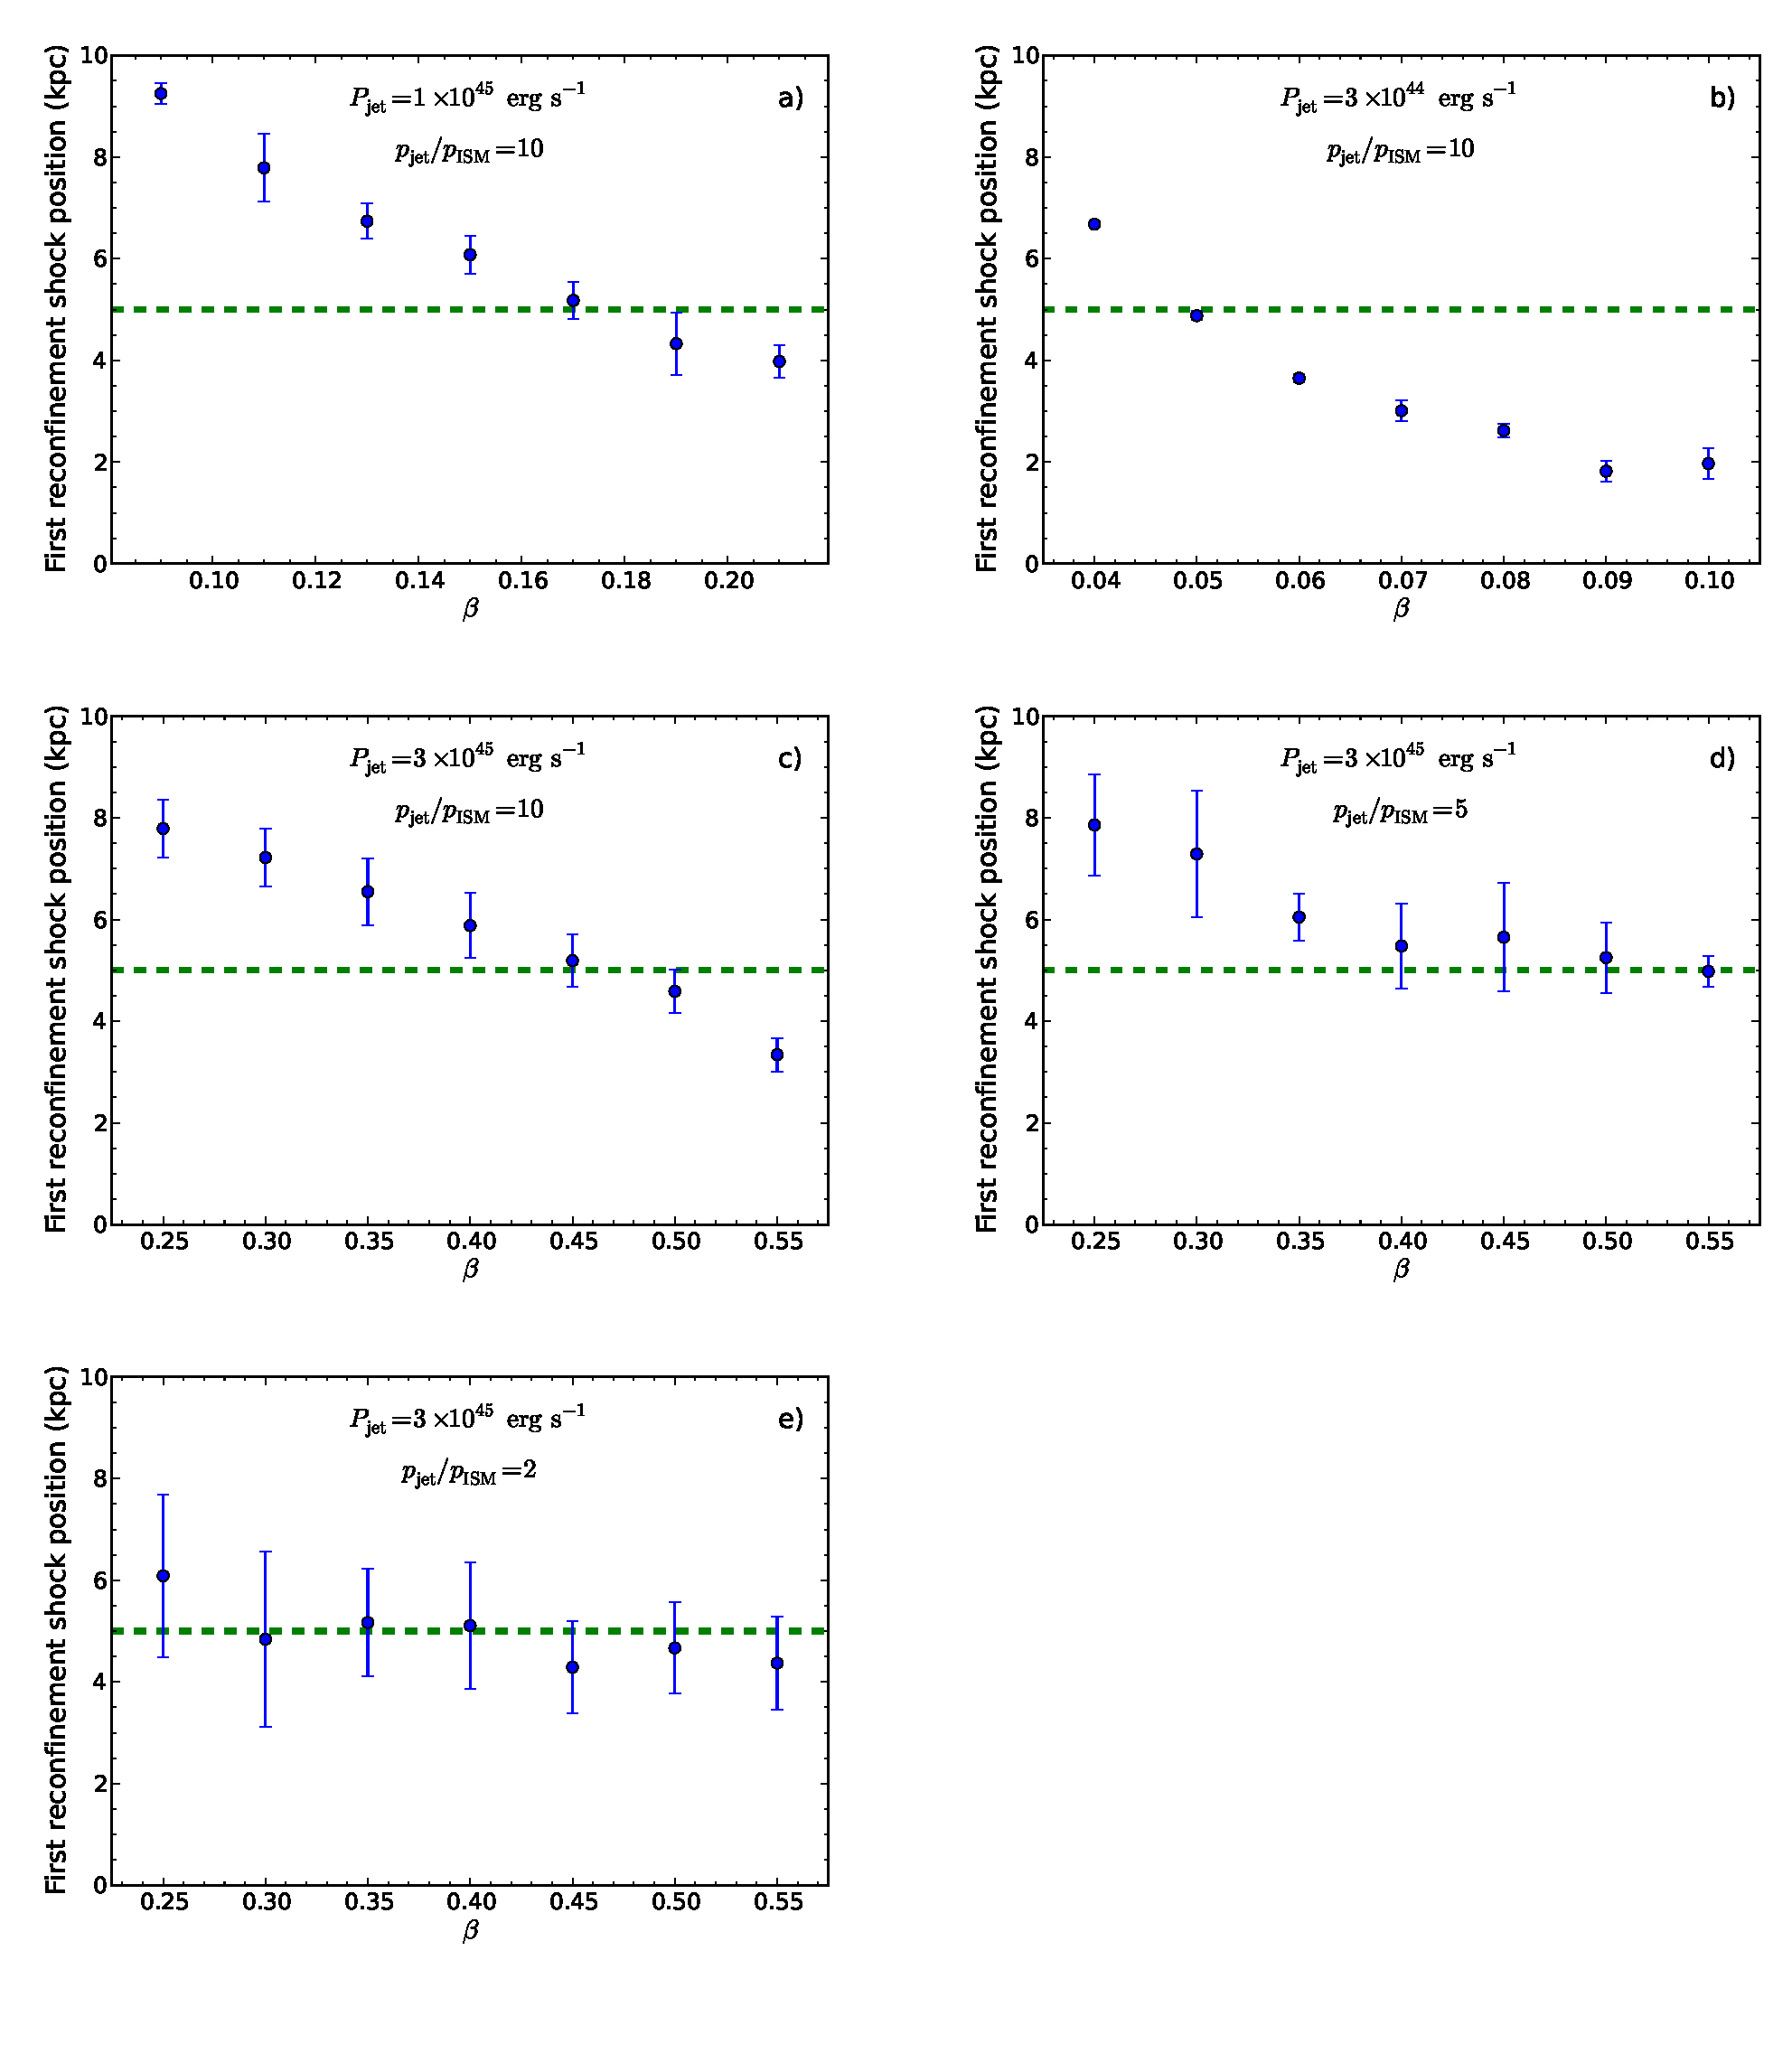
\includegraphics[width=\textwidth]{pps.eps}
\caption{Position of the first  reconfinement shock (Mach disk for significantly over-pressured jets $p_{\rm{jet}}/p_{\rm{a}}=10$ in panel a), b), and c) or the first conical shock for a relatively less over-pressured jet $p_{\rm{jet}}/p_{\rm{a}} = 5$ and 2 in panel d) and e)) as a function of $\beta$, the jet velocity in units of the light speed, measured for three sets of simulations. Each point represents the average of 25 measurements of the position of the Mach disk or first conical shock, which fluctuates with time about a mean value. The error bars represent the standard deviation of the measurements. The dashed green line at $5 \, \rm kpc$ (the first shock is assumed at $6 \, \rm kpc$ and the jet inlet in the simulation is at a distance $\sim 1 \, \rm kpc$ from the galaxy centre) in each panel represents the location of the observed southern edge of the bright knot, which I assume to be either a Mach disk or a conical shock. Measurements are for: a) parameter set A; b) parameter set B, c) parameter set Ca, d) parameter set Cb and e) parameter set Cc. These five relationships along with the assumed location of the Mach disk or the first conical shock in the northern jet at $\sim6$ kpc from the radio core lead to different acceptable jet velocities $0.17\,c$, $0.05\,c$, $0.45\,c$, $0.4-0.55\,c$ and $0.25 - 0.55\,c$ with three different jet kinetic powers $1\times10^{45}$ erg s$^-1$ (our fiducial value), as well as lower and higher values of $3\times10^{44}$ erg s$^-1$, and $3\times10^{45}$ erg s$^-1$.}
\label{mach_position}
\end{figure*}


\subsection{Results of parameter-space study}
\begin{figure}
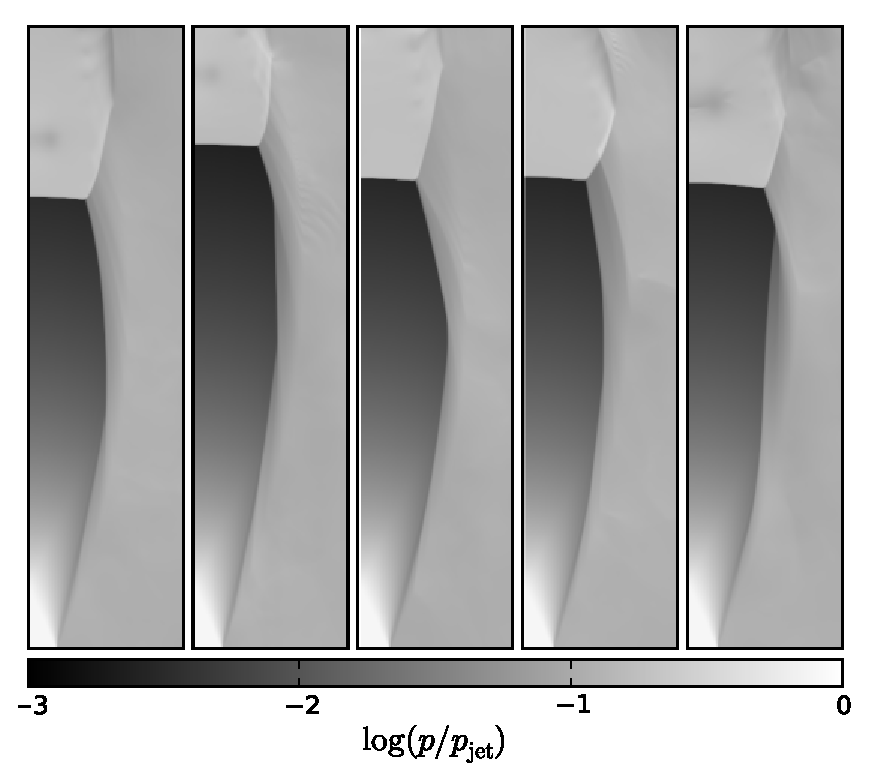
\includegraphics[width=\linewidth]{pml.eps}
\caption{Five snapshots of the logarithmic pressure maps of run Av. The sequence shows the Mach disk moving with time about a mean position. The dimensions of each panel are $2\,\mathrm{kpc}\times8\,\mathrm{kpc}$. The time interval between each snapshots is $100\,\mathrm{kyr}$.}
\label{pressure_evolution}
\end{figure}

The main aim of the parameter space study is to determine the relationship between the position of the first jet shock and jet parameters, in particular, the jet velocity and the jet power. Adopting a shock location at a deprojected distance of $\sim6\,\mathrm{kpc}$ from the core, as inferred from the radio image of Fig.~\ref{taylor} and the assumed inclination angle of
$\theta=42^\circ$ \citep{taylor90}, I use these relationships to constrain the jet velocity of the northern Hydra A jet.

An incentive for this approach comes from the (non-relativistic) expression for the natural wavelength of a supersonic jet, $\Lambda$, with diameter, $D$, and Mach number, $M$, $\Lambda/D = 1.3\sqrt{M^2 - 1}$ \citep{birkhoff57a}.
%\begin{equation}
%\lambda/D = 1.3\sqrt{M^2 - 1}
%\label{mach_position_jet_velocity}
%\end{equation}
This relationship indicates that the spacing of jet shocks should be a function of the Mach number and hence of the velocity of the jet (given that other parameters are constrained by the jet power). I, therefore, vary the jet velocity and at the same time vary the density parameter $\chi$ to maintain a constant jet kinetic power, noting the location of the first jet shock (if one exists) for each run.

In each simulation the positions of shock structures in the jet vary with time. They oscillate about a mean position. For each run, I have therefore measured the position of the jet shock at 25 snapshots with 100 kyr time difference between each two adjacent snapshot. The points in Fig.~\ref{mach_position} show the mean position of the jet shock, and the extent of the oscillation is indicated by the by error bars which represent the standard deviation of the measurements. 

The variations in the shock positions occur because the pressure field in the backflow adjacent to the jet changes continuously as a result of the turbulence in the cocoon. An example of this is shown in Fig. \ref{pressure_evolution} which shows the position of a Mach disk at five different time steps.

Fig. \ref{mach_position} shows the dependence of the distance of the first jet shock from the jet base upon the jet velocity for three different values of the jet kinetic powers: $P_{\rm{jet}}=1\times10^{45} \rm \> erg \> s^{-1}$ (the fiducial value, see \S~\ref{jet_kinetic_power}), $P_{\rm{jet}}=3\times10^{44} \rm \> erg \> s^{-1}$ and $P_{\rm{jet}}=3\times10^{45} \rm \> erg \> s^{-1}$. These are results from the runs in Table~\ref{simulation_parameters} set A, set B, set Ca, set Cb, and Cc respectively. In panels (a), (b) and (c) the first shock is a Mach disk; in panel (d) and (e) the first shock is a conical shock.
Since the jet inlet in the simulation is at a distance $1 \, \rm kpc$ from the centre of the galaxy I locate the first shock at $5 \, \rm kpc$ in each panel to determine the jet velocities. The inferred jet velocities for each result of Fig.~\ref{mach_position} is summarised in Table~\ref{inferred_jet_velocities}.

%For future work I adopt a fiducial value for the Hydra A jet velocity of $0.17c$ and I select Av as the fiducial model for the following reasons. 

\section{Summary and discussion}
Here I summarise the results of the axisymmetric models based on the assumption that the only bright knot, apparent in Fig.~3 of \citet{taylor90}, of the inner 10~kpc Hydra A northern jet, is a consequence of a Mach disk at approximately 6~kpc. 

\begin{enumerate}
\item Among the models with the fiducial jet kinetic power $1\times10^{45}$ erg s$^{-1}$ (set A), the best fit model for Hydra A northern jet (which provide a Mach disk at approximately 6~kpc from the core) is Av. The jet velocity of the best fit model is 0.17~$c$. Using a jet-to-counterjet brightness ratio $R=1.9$ \citep{taylor96}, and an inclination of the source to the line of sight of $\theta = 42^\circ$ \citep{taylor93}, in the formula of Doppler beaming, $R={((1+\beta \cos\theta)/(1-\beta \cos\theta)})^{2-\alpha}$, I estimate a jet velocity 0.17~c. 

Therefore two completely different approaches, one based on the interaction of the jet and the atmosphere and the other based on relativistic Doppler beaming, give the same estimate for the jet velocity of Hydra A jets. However, later, using the 6~cm VLA data of Hydra A I estimate a higher jet-to-counterjet brightness ratio $R = 7$. Attributing this ratio to Doppler beaming I obtain a moderately relativistic jet velocity $\approx 0.5~c$. 

A mild relativistic jet velocity for Hydra A $\approx 0.17~c$ is also inconsistent with the theoretical estimate of jet velocity for FR I radio jets $\approx 0.8~c$ provided by \citep{laing14}.

%For the relativistic beaming estimate, I adopt a jet-to-counterjet brightness ratio $R = 1.9$ and an inclination of the source to the line of sight of $\theta = 42^\circ$ \citep{taylor96,taylor93}. This gives an estimate $\beta\approx0.17$. 

\item In the best fit model (run Av), the density ratio between the jet and the ambient medium is $\eta \approx 10^{-2}$. This density ratio is relatively higher than the typical assumption light AGN jets $\eta \approx 10^{-4}$. This relatively heavy jet can be attributed to the entrainment of the pc~scale jets with a heavy gas (\citet{dwarakanath95} detected HI gas near the core of Hydra A galaxy)near the core.

\item In model Av the internal Faraday rotation $\Psi_{20 \rm cm} = 1.42$ is also high, which is inconsistent with the observed polarisation of the jet \citep{taylor93}. Three possible explanation for this uncomfortably high value of $\Psi_{20 \rm cm}$ are: i) Equipartition between the magnetic field energy in the radio plasma and the particle energy does not obtain. The magnetic field may be less than the equipartition value, which would imply lower internal Faraday rotation; ii) A preferentially perpendicular orientation of the magnetic field with respect to the line of sight, e.g. due to a toroidal magnetic field, will give smaller values of the rotation measure. c) For random magnetic field distributions in the radio plasma, the rotation measure is decreased by a factor of $N^{1/2}$, where $N$ is the number of magnetic field reversals across the jet. 

\item If lower jet kinetic powers are assumed, the best values for the jet velocity require values of the density parameter $\chi$ that are uncomfortably large, e.g., in the case in which $P_\mathrm{jet}=3\times10^{44}\,\mathrm{erg}\,\mathrm{s}^{-1}$, $\beta=0.04$ and $\chi=3143$ (run Bi) give the best fit for the location of the jet shock. In this case the internal Faraday rotation at 20~cm is 17.76~radians, clearly inconsistent with the polarisation of the jets.

\item The scenario of higher jet kinetic power and a comparatively less over-pressured jet suggest (runs Civb, Cvb, Cvib and Cviib) a range of jet velocity from $\sim0.45$ c to $\sim0.55$ c. In the case of higher jet kinetic power and a nearly pressure equilibrium jet (runs Cic to Cviic) a mildly decreasing trend of the first conical shock position with increasing jet velocity indicates an wide range of possible jet velocities from $\sim0.25$ c to $\sim0.55$ c. These two cases involve conical shocks so that the jet remains supersonic after the first shock. 

%Large value of the jet density parameter $\chi = 116$ in this model is consistent with the inferred value of $k \sim 10$ for the Hydra A radio lobes.  
%\item 

%The only parameter with unusual values in model Av is the internal Faraday rotation $\Psi_{20 \rm cm} = 1.42$, which is inconsistent with the observed polarisation of the jet \citep{taylor93}. Three possible explanation for this uncomfortably high value of $\Psi_{20 \rm cm}$ are: i) Equipartition between the magnetic field energy in the radio plasma and the particle energy does not obtain. The magnetic field may be less than the equipartition value, which would imply lower internal Faraday rotation; ii) A preferentially perpendicular orientation of the magnetic field with respect to the line of sight, e.g. due to a toroidal magnetic field, will give smaller values of the rotation measure. c) For random magnetic field distributions in the radio plasma, the rotation measure is decreased by a factor of $N^{1/2}$, where $N$ is the number of magnetic field reversals across the jet. 
%
%
%\item Higher jet kinetic powers and a significantly over-pressured jet lead to a higher estimate for the jet velocity, e.g., for $P_\mathrm{jet}=3\times10^{45}$ erg s$^{-1}$, the estimated jet velocity is $\beta \approx 0.45$ (run Cva), which implies a brightness ratio between the northern and southern jets due to relativistic beaming $\approx 5$, a factor of 2.5 larger than that seen in the data \citep{taylor96}. 
%Notwithstanding the inconsistency with relativistic beaming estimates, these
%models merit further investigation in three dimensions because of the observation of possible shock structures inside the northern lobe, indicative of supersonic flow there. 
\end{enumerate}

As I stated in the beginning of the chapter, the results presented here are based on the study of the contour image of the northern jet presented in \citep{taylor90}. A careful study of the original data (which was used to produce Fig.3 of \citet{taylor90}) shows that a fainter knot is also apparent near the core (see Fig.~\ref{northern}). Therefore, in the following chapter I revised my study of the Hydra A northern jet with a further improvement of the axisymmetric model. 

Although the models presented here are inappropriate to the Hydra A northern jet and provide unusual values for the jet velocity, the density ratio of the jet and the ambient medium and the internal Faraday rotation, they shed some light on the physics of the jet-ICM interaction. For example, 

\begin{enumerate}
\item Formation of different reconfinement shocks, diamond shocks or normal shocks, depending on the pressure ratio between the jet and the ambient medium (see Fig.~\ref{pressure_comparison}). 
\item Formation of two different jet-lobe morphologies: one is a lobe fed by a jet with biconical shocks and the other is a lobe fed by a jet with a disruptive Mach disk (see \S~\ref{morphological_structure} and Fig.~\ref{shock_comparison})
\item A correlation between the jet velocity and the location of the inner jet knot. This correlation can be easily demonstrated by the relationship between the jet kinetic power $P_{\rm jet}$ and Mach number $M_{\rm}$ for a non-relativistic flow provided by \citet{sutherland07}:
\begin{equation}
P_{\rm jet} = \frac{\gamma}{\gamma - 1} p_{\rm jet} v_{\rm jet}A_{\rm jet} \left ( 1 + \frac{\gamma -1 }{2} M_{\rm}^2 \right )
\label{e:nrP}
\end{equation}
and the relationship between the shock spacing and the Mach number of the jet (equation \ref{e:birkhoff}):
\begin{equation}
\Lambda/D = 1.3\sqrt{M^2 - 1} \nonumber
\end{equation}
According to the later equation, for a lower shock spacing we require lower Mach number. Then the former equation implies that, for a fixed jet kinetic power, jet pressure and jet inlet radius, lowering the Mach number results an increase in the jet velocity. Hence there is an inverse relationship between the shock spacing and the jet velocity. This relationship suggests that the appearance of a bright knot near the core may be a remedy of the unusual low velocity for Hydra A jets. 

In the following chapter, based on two knots in the inner 10~kpc of Hydra A northern jet, I estimate a jet velocity $\approx 0.8~c$, which is theoretically reasonable for a FRI source \citep{laing14}. 

\item The Mach number of the jet is related to the jet velocity $v_{\rm jet}$, the jet pressure $p_{\rm jet}$ and the jet density $\rho_{\rm jet}$:
\begin{equation}
M = v_{\rm jet} \rho_{\rm jet}/ \gamma p_{\rm jet}.
\end{equation} 
According to equation~\ref{e:nrP} a fixed jet kinetic power, jet pressure and jet inlet radius, increase in the jet velocity results a decrease in the jet density and hence a decrease in the Faraday rotation of the source. Therefore, as above, the bright knot near the core will provide lower values of jet density and Faraday rotation. In the next chapter, modelling the Hydra A jet knot with two bright knots, I obtain a density ratio between the jet and the ambient medium $\eta \approx 10^{-4}$, which is a typical value of an AGN jet, and a Faraday rotation $\Phi \approx 10^{-2}$, which is comfortably less than unity and consistent with the observed polarisation of the jet \citep{taylor93}.
\end{enumerate}


 


%%%%%%%%%%%%%%%%%%%%%%%%%%%%%%%%%%%%%%%%%%%%%%%%%%%%%%%%%%%%%%%%%%%%%%%%
% 
%												Discussion and Summary
%
%%%%%%%%%%%%%%%%%%%%%%%%%%%%%%%%%%%%%%%%%%%%%%%%%%%%%%%%%%%%%%%%%%%%%%%%

%\section{Summary and Discussion} \label{discussion}
%
%
%The key features of the radio jets of Hydra A, which I seek to explain in this paper are the bright knot in the northern jet at $\sim6$ kpc from the core and the turbulent transition of both northern and southern jets to plume like structures at $\sim10$ kpc as evident in the radio image (see Fig.~\ref{taylor}). To this end, I have performed a series of two dimensional axisymmetric relativistic hydrodynamic simulations of the dynamical interaction of the Hydra A jets with their environment. 
%
%%% aln %%gvb
%To ensure that I use reasonable values for the jet parameters in the simulations, I have estimated the powers associated with the inner X-ray cavities of Hydra~A corresponding to the inner radio lobes utilising the 4.6~GHz radio data \citep{taylor90} and have compared them with the estimates of \citet{wise07} for the same cavities based on the X-ray data. I obtain a power of each inner cavity $\sim 10^{44} \> \rm ergs \> s^{-1}$ consistent with their estimate $\sim 2 \times 10^{44} \> \rm ergs \> s^{-1}$ within a factor of 2. Hence, I adopt their estimate of the total jet power $\sim 10^{45} \> \rm ergs \> s^{-1}$ as the fiducial value for the numerical simulation. To obtain the X-ray atmosphere profiles surrounding the Hydra A radio source within 10 kpc of the core, I have fitted and extrapolated the X-ray data from \citet{david01} towards the centre of the galaxy.
%
% 
%On the basis of the minimum pressure estimates I conclude that the parameter $k \sim 10$. High values of this parameter are supported by other recent studies: \citet{birzan08} estimated $k$ for a group of radio galaxies assuming that the radio lobes are in pressure equilibrium with the ambient medium. Their estimates include the Hydra A radio lobes at 1.4 GHz for which they obtained a value of $k \approx 13$. \citet{hardcastle10} studied the inverse-Compton X-ray emission from the outer Hydra A radio lobes and obtained values of $k \sim 17$ and 23 for minimum Lorentz factor cut-offs of $\gamma_1=1$ and 10 respectively.  
%
%Our simulation results support the idea that a Mach disk is responsible for the bright knot in the northern jet at a deprojected distance of $\sim 6$ kpc from the core. The abrupt turbulent transition of the northern jet would then be caused by the rapid deceleration of the jet following the Mach disk. In contrast, the gradual transition of the southern jet to a turbulent plume could be mediated by less disruptive, conical reconfinement shocks. However, as I have noted, this interpretation needs to be confirmed by further three dimensional simulations.
%
%Simulation Av, for which $P_{\rm{jet}}=1\times10^{45} \> \rm erg \> s^{-1}$, is the fiducial model for the inner 
%$\sim 10$ kpc radio structure of Hydra A. As expected of a jet over-pressured with respect to its environment by a factor of 10, the jet in run Av produces a Mach disc at the first reconfinement shock. The Mach disk remains quasi-stationary at $\sim 5$ kpc from the base of the jet over at least $24$ Myr.
%The jet flow in run Av is violently disrupted at the Mach disk, following which it decelerates rapidly toward a transition to turbulence at $\sim10$ kpc from the core. This matches with the observed location of the beginning of the turbulent plume in the northern region of Hydra A. The jet velocity $\beta=0.17$ for run Av is implied by the relationship between Mach disk position and jet velocity obtained from the parameter space study. 
%
%Using the jet to counter-jet brightness ratio determined by \citet{taylor96} and a jet inclination angle $\theta \approx 48^\circ$ inferred by \citet{taylor93a} from the rotation measure asymmetry I estimate a jet velocity $\approx 0.17\,c$ from standard Doppler beaming theory. Thus, two completely different approaches, one based on the dynamical interaction of the jets with the atmosphere and the other based on relativistic Doppler beaming, give the same estimate for the jet velocities. 
%
%We have also used the analytical theory developed by \citep{stawarz06} to estimate the position of the reconfinement shocks of the Hydra A jets. Adopting parameters from run Av, I find a distance to the first reconfinement shock of 7.5 kpc for a non-relativistic particle dominated jet and 18 kpc for relativistic-particle dominated jets, supporting the previous conclusions that the jets are thermally dominated. This suggests that the jets have efficiently entrained material at small radii, for example, in the region of HI clouds near the core. The interactions with parsec scale HI clouds are well below the resolution of the simulations, but warrant further investigation.
%
%One concern with the fiducial model is that the value of the internal Faraday rotation $\Psi_{20} = 1.42$, is uncomfortably large,in view of the fact that the jets are polarised at 20~cm \citep{taylor93}. However, these estimates are maximal and would be lower if the magnetic field were sub-equipartition, if the angle between the magnetic field and line of sight were large or if there are a large number of field reversals. 
% 
%Our models of Hydra A and its associated environment can explain prominent jet features of the inner 50 kpc including the bright knot on the northern side and the turbulent transition on both sides. However, the Hydra A inner jets are bent in contrast to the straight structures that I have modelled so far, using an axisymmetric approximation. For the northern jet, the curvature within 10 kpc is modest, and we expect an approximation by a straight jet to be reasonable. The existence of the  bright knot within the plume region on the southern side of the radio source, is most likely related to a shock produced by the supersonic jet flow as it deflected through more than the Mach angle off the wall of the cavity produced by the radio plasma (see Fig.~\ref{taylor}). A realistic model for this knot cannot neglect the curvature of the jet, requiring three-dimensional numerical simulations.
%
%The next paper in this series will focus on modelling the curvature of both jets and the details of the transition from jets to plumes. In the third paper of this series I will present a full three-dimensional model of the the X-ray and radio emission of Hydra A.
